\documentclass{../TexTemplate/myslide}
\usepackage[slide,table,cpp]{../TexTemplate/mypackage}
\hypersetup{colorlinks=true,linkcolor=black,urlcolor=blue}

\usepackage[cache=false]{minted}
\newminted{bash}{frame=single}

\title[ToolsSeminar]{Tools Seminar}
\subtitle{Week 3 - C/C++ Toolchain}
\author[chhzh123]{Hongzheng~Chen}
\date[Nov 29, 2019]{Nov 29, 2019}

\begin{document}

\begin{frame}
\titlepage
\end{frame}

\begin{frame}
\tableofcontents
\end{frame}

\section{Computer System Overview}
\begin{frame}
\sectionpage
\end{frame}

\begin{frame}{Some Introductory Books \& Courses You Need to Know}
\href{https://eecs.berkeley.edu/resources/undergrads/cs/degree-reqs-lowerdiv}{UC Berkeley} CS Major Lower Division Degree Requirements (61 Series)
\begin{itemize}
	\item 61A: \href{https://cs61a.org/}{Structure and Interpretation of Computer Programs}
	\item 61B: \href{https://inst.eecs.berkeley.edu/~cs61b/fa19/}{Data Structures}
	\item 61C: \href{https://cs61c.org/}{Great Ideas in Computer Architecture (Machine Structures)}
\end{itemize}
\href{http://catalog.mit.edu/degree-charts/computer-science-engineering-course-6-3/}{MIT EECS} General Institute Requirements
\begin{itemize}
	\item 6.001: \href{https://ocw.mit.edu/courses/electrical-engineering-and-computer-science/6-001-structure-and-interpretation-of-computer-programs-spring-2005/}{Structure and Interpretation of Computer Programs}\\\quad $\to$ 6.0001 Python
	\item 6.006: \href{https://courses.csail.mit.edu/6.006/fall11/notes.shtml}{Introduction to Algorithms}
	\item 6.004: \href{https://6004.mit.edu/web/fall19/}{Computation Structures}
\end{itemize}
\end{frame}
% https://zhuanlan.zhihu.com/college-simulator

\begin{frame}{Some Introductory Books \& Courses You Need to Know}
\begin{figure}
\begin{tabular}{ccc}
\href{https://mitpress.mit.edu/sites/default/files/sicp/full-text/book/book.html}{SICP} & \href{https://en.wikipedia.org/wiki/Introduction_to_Algorithms}{CLRS} & \href{https://csapp.cs.cmu.edu/}{$\star$CS:APP}\\
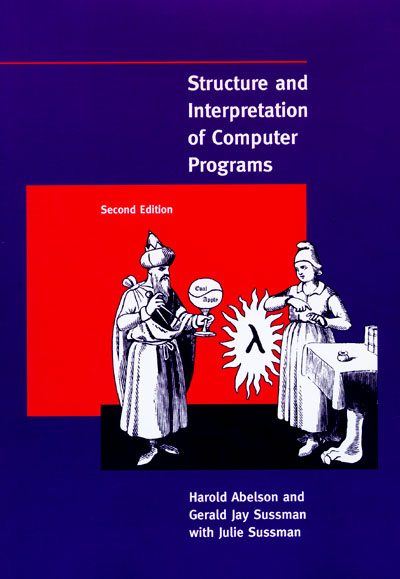
\includegraphics[width=0.3\linewidth]{fig/sicp.jpg} &
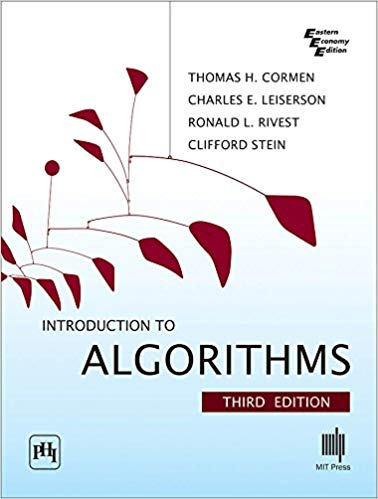
\includegraphics[width=0.3\linewidth]{fig/clrs.jpg} &
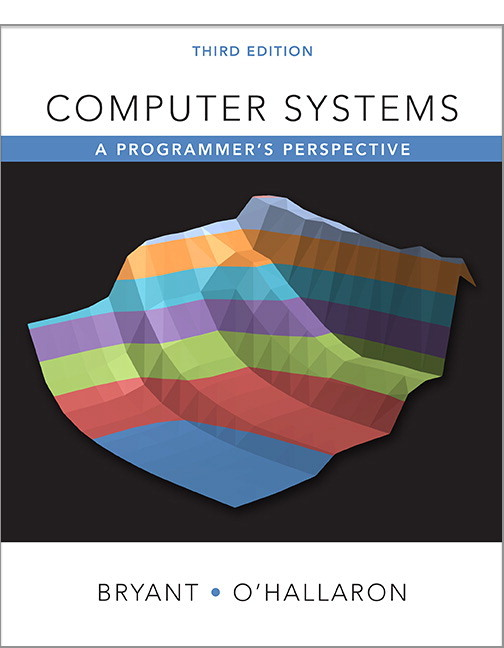
\includegraphics[width=0.3\linewidth]{fig/csapp.jpg}
\end{tabular}
\end{figure}
\end{frame}

\begin{frame}
\begin{figure}
\centering
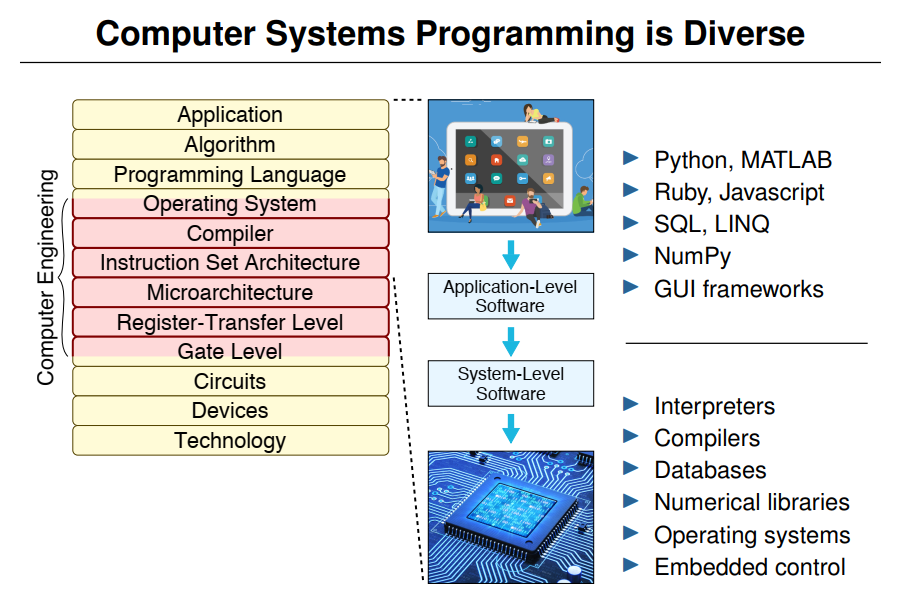
\includegraphics[width=0.9\linewidth]{fig/computer_system_stack.png}
\caption*{\scriptsize Source: Christopher Batten, \emph{\href{https://www.csl.cornell.edu/courses/ece2400/handouts/ece2400-overview.pdf}{Cornell ECE 2400}: Computer Systems Programming}, Fall 2019}
\end{figure}
\end{frame}
% https://www.microcontrollertips.com/a-look-at-the-computer-engineering-stack/

\section{C/C++ Programming Language}
\begin{frame}
\sectionpage
\end{frame}

\subsection{C/C++ Introduction}
\begin{frame}
\subsectionpage
\end{frame}
\begin{frame}{TIOBE Ranking}
Nov 2019 Ranking
\begin{figure}
\centering
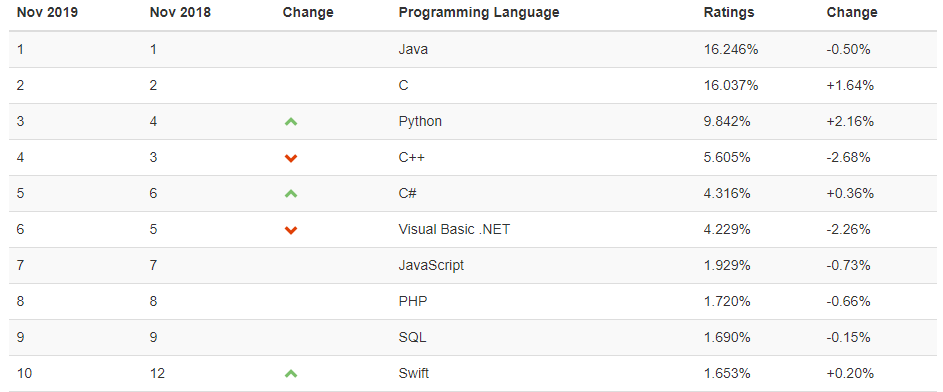
\includegraphics[width=\linewidth]{fig/TIOBE.png}
\caption*{\scriptsize Source: \url{https://www.tiobe.com/tiobe-index/}}
\end{figure}
\end{frame}

\begin{frame}{C Programming Language}
Actually in 9102, most of the CS top schools in US use Python as their introductory language.
\pause
\bigskip
\begin{center}
\large So why we still use C?
\end{center}
\end{frame}

\begin{frame}{C Programming Language}
\begin{itemize}
	\item Speed: Very close to hardware, extremely fast\\
	$\to$ $^\star$High performance computing (HPC)
	\begin{itemize}
		\item Parallel computing: OpenMP, MPI
		\item Specific accelerator: cuda, Verilog
	\end{itemize}
\end{itemize}
\begin{figure}
\centering
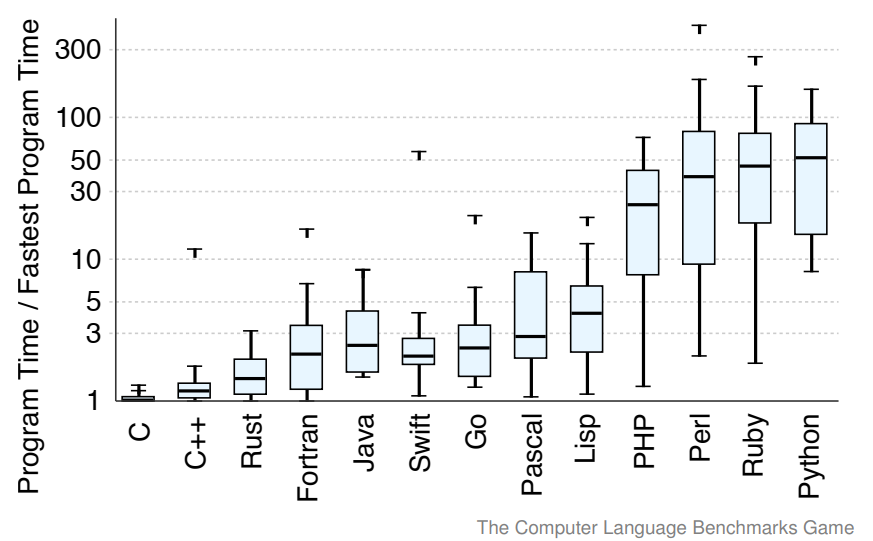
\includegraphics[width=0.6\linewidth]{fig/running_time.png}
\end{figure}
\end{frame}

\begin{frame}{C Programming Language}
\begin{itemize}
	\item Portability:
	\begin{itemize}
		\item OS
		\item Networking
		\item Embedded systems
	\end{itemize}
	\item Stability: Static type \& rigorous spec
	\begin{itemize}
		\item Compiler / Interpreter
	\end{itemize}
\end{itemize}
\end{frame}

\begin{frame}{C Programming Language}
C influences lots of PLs which all has C-like grammar (Java, C\#)
\begin{figure}[H]
\centering
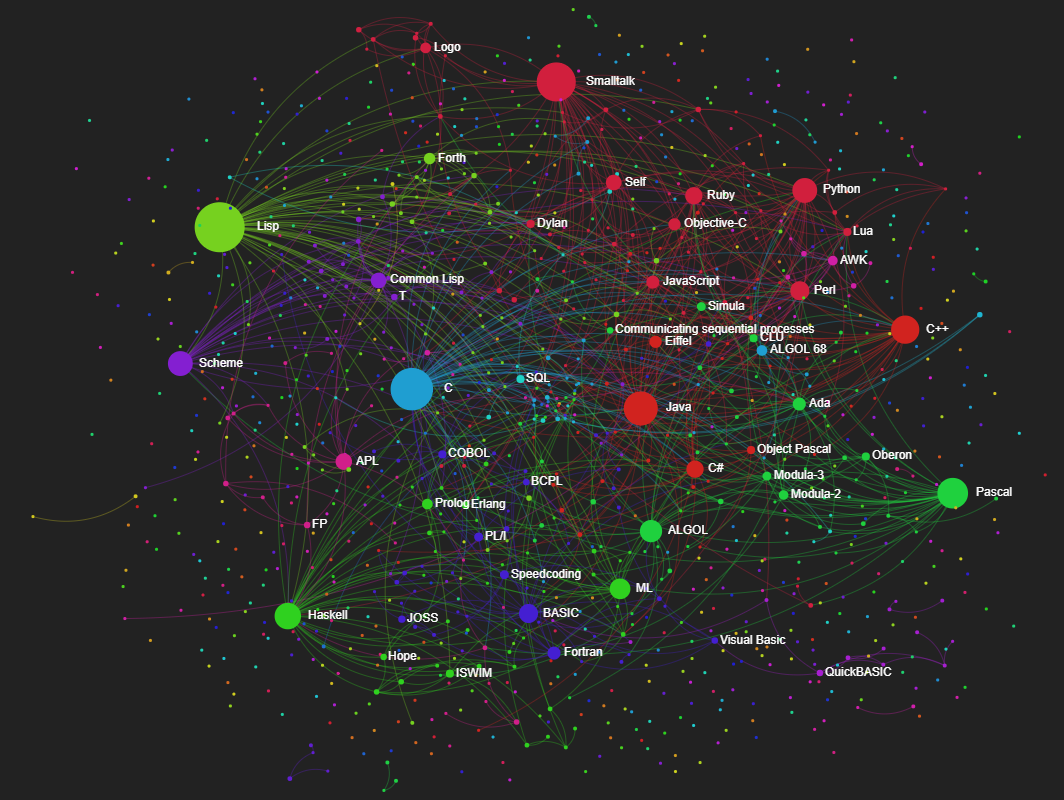
\includegraphics[width=0.7\linewidth]{fig/pl_influence_network.png}
\caption*{\scriptsize Source: \href{https://exploring-data.com/vis/programming-languages-influence-network/}{Programming Languages Influence Network}}
\end{figure}
\end{frame}

\begin{frame}{So what about C++?}
\begin{itemize}[<+->]
\item Superset of C, but not only C
\begin{center}
\Large\textcolor{red}{\textbf{C++ $\ne$ C + STL!}}
\end{center}
\item Object-Oriented Programming (OOP) support
\begin{itemize}
	\item \textbf{Abstraction \& Encapsulation}
	\item Enable to distribute works in a large project
\end{itemize}
\item Modern language features
\begin{itemize}
	\item Templates and Generic Programming: Polymorphism
	\item C++11 standard
\end{itemize}
\item Also lightweight, fast, and high-performance
\end{itemize}
\end{frame}

\subsection{Compiling and Running C/C++}
\begin{frame}
\subsectionpage
\end{frame}

\begin{frame}{Some Compilers for C/C++}
\begin{itemize}
\item gcc/g++: GNU Compiler Collection
\begin{itemize}
	\item \href{http://www.mingw.org/}{MinGW} (Minimalist GNU for Windows)
\end{itemize}
\item clang/clang++
\begin{itemize}
	\item Low Level Virtual Machine (LLVM) [UIUC, CGO'04]
	\item $\to$ commonly used for building your own compiler for DSL
\end{itemize}
\item Visual Studio C++
\begin{itemize}
	\item Mainly for Windows applications development
\end{itemize}
\item icc/\href{https://software.intel.com/en-us/c-compilers}{icpc}: Intel C/C++ Compiler
\begin{itemize}
	\item Extremely high-performance when compiling to Intel CPU architecture
	\item Need a student account
\end{itemize}
\end{itemize}
\end{frame}

\begin{frame}[fragile]{Four stages of Compilation}
\begin{columns}
\begin{column}{0.5\linewidth}
\tiny
\begin{minted}[frame=single]{cpp}
// hello.c
#include <stdio.h>

int main(void) {
    printf("Hello world!\n");
    return 0;
}
\end{minted}
\tiny
\begin{minted}[frame=single]{gas}
; hello.s
.LC0:
    .string "Hello world!"
main:
    ; protect state
    push    rbp
    mov     rbp, rsp
    ; call function
    mov     edi, OFFSET FLAT:.LC0
    call    puts
    ; restore state & return
    mov     eax, 0
    pop     rbp    
    ret
\end{minted}
\end{column}
\begin{column}{0.5\linewidth}
\begin{center}
\begin{tikzcd}
\text{\textit{hello.c}}\arrow{d}{\text{\textcolor{red}{Preprocessing}}}\\
\text{\textit{hello.i}}\arrow{d}{\text{\textcolor{red}{Compilation}}}\\
\text{\textit{hello.s}}\arrow{d}{\text{\textcolor{red}{Assembly}}}\\
\text{\begin{tabular}{c}\textit{hello.o(bj) + printf.o}\\(Binary)\end{tabular}}\arrow{d}{\text{\textcolor{red}{Linking}}}\\
\text{\textit{hello}}
\end{tikzcd}
\end{center}
\end{column}
\end{columns}
\end{frame}
% https://www.calleerlandsson.com/the-four-stages-of-compiling-a-c-program/

\begin{frame}[fragile]{Preprocessing}
Try this:
\begin{lstlisting}
// student.c
#include "name.txt"
#include "number.txt"
\end{lstlisting}
Use C preprocessor (\verb'cpp') to generate output
\begin{bashcode}
$ cpp student.c -o student.out
$ cat student.out
\end{bashcode}
% $ cpp student.c -P -o student.out
\end{frame}

\begin{frame}[fragile]{Preprocessing}
You can include several times
\begin{lstlisting}
#include "name.txt"
#include "name.txt"
#include "name.txt"
#include "number.txt"
#include "number.txt"
#include "number.txt"
\end{lstlisting}
But it's very dangerous due to dependency $\to$ function redefinition
\end{frame}

\begin{frame}[fragile]{Preprocessing}
Make sure the file is only included once:
\begin{lstlisting}
#ifndef NAME_TXT
#define NAME_TXT
Alice
Bob
Carlo
#endif // NAME_TXT
\end{lstlisting}
\pause
* Preprocessor macros are very ugly! C++20 proposes Modules (\verb'import')
\end{frame}

\begin{frame}[fragile]{Compilation \& Assembly}
\begin{minted}[frame=single]{bash}
$ gcc avg.c -c -o avg.o
$ objdump -dC avg.o
\end{minted}
\begin{itemize}
	\item Online editor and compiler: \href{https://repl.it/}{Repl.it}
	\item Online assembly code generation: \href{https://godbolt.org}{GodBolt}
\end{itemize}
\scriptsize Ref: \href{https://cornell-ece2400.github.io/ece2400-docs/ece2400-sec2-c-basics/}{ECE 2400}
\end{frame}

\begin{frame}[fragile]{Linking}
\begin{minted}[frame=single]{bash}
$ gcc avg.o -o avg
\end{minted}
\begin{itemize}
	\item Static library: \verb'.a' (Linux), \verb'.lib' (Windows)
	\item Dynamic library: \verb'.so' (Linux), \verb'.dll' (Windows)
\end{itemize}
\begin{figure}
\centering
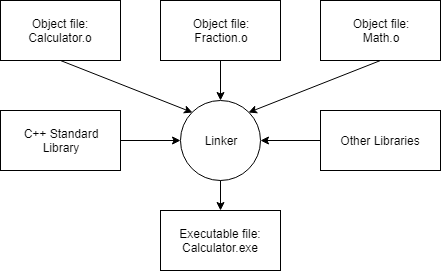
\includegraphics[width=0.5\linewidth]{fig/linking.png}
\caption*{\scriptsize Source: \href{https://www.learncpp.com/cpp-tutorial/introduction-to-the-compiler-linker-and-libraries/}{LearnCpp}}
\end{figure}
\end{frame}

\begin{frame}[fragile]{Compilation Flags}
When you configure C environment in VS Code, you need to add them
\begin{itemize}
	\item \verb'-o': output to file
	\item \verb'-O': \verb'-O0', \verb'-O1', \verb'-O2', \verb'-O3' (See \href{https://gcc.gnu.org/onlinedocs/gcc/Optimize-Options.html}{gcc optimization options})
	\item \verb'-Wall': with all warnings
	\item \verb'-Werror': all warnings to errors
	\item \verb'-D[FLAG]' or \verb'-D[FLAG]=VALUE': pass preprocessor flag \verb'#if FLAG ...'
	\item \verb'-std=c++11': standard
	\item \verb'-I': [/path/to/header-files] (\verb'.h', \verb'.hpp')
	\item \verb'-L': [/path/to/shared-libraries]
	\item \verb'-l': Links to shared library or shared object (\verb'.so', \verb'.dll')
\end{itemize}
\scriptsize Ref: \url{https://caiorss.github.io/C-Cpp-Notes/compiler-flags-options.html}
\end{frame}

\subsection{Auto Building}
\begin{frame}
\subsectionpage
\end{frame}

\begin{frame}{Existing Problems}
\begin{itemize}
\item Programs with hard dependency, say projects with 100k LoC
\item Intractable to enter a bunch of commands
\item Some unmodified files will be regenerated
\end{itemize}
\pause
\begin{center}
\large We need \textbf{auto compilation} tools!
\end{center}
\end{frame}

\begin{frame}[fragile]{Makefile}
Put previous commands together
\begin{minted}[frame=single]{make}
avg: avg.o
	gcc avg.o -o avg

avg.o: avg.c
	gcc avg.c -c -o avg.o
\end{minted}
Just type \verb'make'!
\end{frame}

\begin{frame}[fragile]{Makefile - Grammar}
\begin{minted}[frame=single]{make}
target : prerequisite0 prerequisite1 prerequisite2
<TAB>command
\end{minted}
\begin{itemize}
	\item First finish \verb'prerequisite'
	\begin{itemize}
		\item If pre does not change, skip it
		\item If pre changes, re-generate it
	\end{itemize}
	\item When all the pre are finished, do \verb'command'
	\begin{itemize}
		\item Can be ANY Linux command!
	\end{itemize}
\end{itemize}
\end{frame}

\begin{frame}[fragile]{Makefile - Variables}
\begin{minted}[frame=single]{make}
CC = gcc

avg: avg.o
	$(CC) avg.o -o avg

avg.o: avg.c
	$(CC) avg.c $(FLAGS) -c -o avg.o
\end{minted}
\end{frame}

\begin{frame}[fragile]{Makefile - Auto Variables}
\begin{itemize}
	\item \verb'$@': Target file
	\item \verb'$^': all prerequisite
	\item \verb'$<': The first prerequisite
	\item \verb'%': wildcard
\end{itemize}
\begin{minted}[frame=single]{make}
CC = gcc
FLAGS = -O3

% : %.c
	$(CC) $(FLAGS) $< -o $@
\end{minted}
Compared with
\begin{minted}[frame=single]{bash}
avg: avg.c
	$(CC) avg.c $(FLAGS) -o avg.o
\end{minted}
\end{frame}

\begin{frame}[fragile]{Makefile - .PHONY}
\begin{minted}[frame=single]{make}
.PHONY : clean
clean :
	-rm edit $(objects)
\end{minted}
\begin{itemize}
	\item \verb'.PHONY': not associated with physical files; target is always out-of-date
	% https://stackoverflow.com/questions/2145590/what-is-the-purpose-of-phony-in-a-makefile
	\item Put it at the back of Makefile
\end{itemize}
\scriptsize * For complete usage of Makefile,\\
\quad please refer to \url{https://chhzh123.github.io/2019-02-24-makefile/}
\end{frame}

\begin{frame}[fragile]{CMake}
\begin{minted}[frame=single]{cmake}
cmake_minimum_required(VERSION 2.8)
enable_language(C)
add_executable( avg avg.c )
\end{minted}
Need to install CMake first (\verb'apt-get install')
\begin{minted}[frame=single]{bash}
$ cmake .
$ make target
\end{minted}
\end{frame}

\subsection{Debugging}
\begin{frame}
\subsectionpage
\end{frame}

\begin{frame}[fragile]{Debugging}
The GNU Debugger (GDB)\footnote{\scriptsize source: \href{https://en.wikipedia.org/wiki/GNU_Debugger}{Wiki}}
\begin{itemize}
\item \verb'gcc -g': Add debug flag
\item \verb'gdb program': Debug \verb'program' (from the shell)
\item \verb'run -v': Run the loaded program with the parameters
\item \verb'bt': Backtrace (in case the program crashed)
\item \verb'info registers': Dump all registers
\item \verb'break 10': Breakpoint at line 10
\end{itemize}
\end{frame}

\begin{frame}{Debugging}
Demo by \emph{Yucheng Chen}
\begin{itemize}
	\item DFS
	\item BFS
\end{itemize}
\end{frame}

\subsection{Testing}
\begin{frame}
\subsectionpage
\end{frame}

\begin{frame}[fragile]{CTest}
\begin{lstlisting}
#include <stdio.h>
#include "avg.h"
#include "utst.h"

int main()
{
  UTST_ASSERT_INT_EQ( avg( 10, 20 ), 15 );
  return 0;
}
\end{lstlisting}
\end{frame}

\begin{frame}[fragile]{CTest}
\begin{minted}[frame=single]{cmake}
cmake_minimum_required(VERSION 2.8)
enable_language(C)
enable_testing()

add_executable( avg avg.c )
add_executable( avg-test avg-test.c )
add_test( avg-test avg-test )
\end{minted}
Type
\begin{minted}[frame=single]{bash}
$ make avg-test
$ make test
\end{minted}
Change the number and regenerate it
\end{frame}

\begin{frame}[fragile]{Other Tools}
\begin{itemize}
	\item Google Unit Test: \href{https://github.com/google/googletest}{Google Test}
	\item Code Coverage: \verb'gcov'
	\item Continuous Integration: \href{https://travis-ci.org/profile}{Travis-CI}, \href{https://codecov.io/}{Codecov.io}
\end{itemize}
\end{frame}

\subsection{Profiling}
\begin{frame}
\subsectionpage
\end{frame}

\begin{frame}[fragile]{Profiling}
Timing:
\begin{itemize}
\item \verb'<time.h>'
\scriptsize
\begin{minted}[frame=single]{cpp}
void timing()
{
    time_t start,stop;
    start = time(NULL);
    foo(); // do something
    stop = time(NULL);
    printf("Time:%ld\n",(stop-start));
}
\end{minted}
\normalsize
\item \verb'time <command>'
\begin{itemize}
	\item \textbf{Real}: Wall clock time - time from start to finish of the call
	\item User: Amount of CPU time spent in user-mode code (outside the kernel)
	\item Sys: Amount of CPU time spent in the kernel
\end{itemize}
% https://stackoverflow.com/questions/556405/what-do-real-user-and-sys-mean-in-the-output-of-time1
\end{itemize}
\end{frame}

\begin{frame}{Profiling}
\begin{itemize}
\item \href{http://www.brendangregg.com/perf.html}{perf} (Linux): CPU, cache, memory etc.
\item \href{https://github.com/opcm/pcm}{pcm} (Intel): CPU, cache, memory etc.
\item \href{http://www.valgrind.org/}{valgrind} [PLDI'07]: memory management
\end{itemize}
\end{frame}

\section{Summary}
\begin{frame}
\sectionpage
\end{frame}

\begin{frame}{Week 2 - C/C++ Toolchain}
\begin{itemize}
	\item Compiling: gcc, clang
	\item Auto building: Makefile, CMake
	\item Debugging: gdb
	\item Testing: CTest
	\item Profiling: time, perf, valgrind
\end{itemize}
\end{frame}

\end{document}